\documentclass{article}
\usepackage{graphicx} % Required for inserting images
\usepackage{listings}
\usepackage{url}
\usepackage[margin=2.5cm]{geometry}
\usepackage{bm}

\usepackage[utf8]{inputenc}
\usepackage[english]{babel}
\usepackage{natbib}





\title{Imperial Project Report \\ 
Cryptography: From Caesar to Quantum}
\author{Eden Zan, Edward Ștefan Bujdei, Amit Paul, Tom Ballantyne}
\date{November 2024}

\begin{document}

\maketitle

\tableofcontents

\section{Introduction}

\subsection{Caesar Cipher}
Encryption methods have been around for thousands of years as a way to communicate information without the risk of being read by unwanted people if it is intercepted. One of the earliest and simplest methods of encryption was the Caesar Cipher, used by Julius Caesar himself. It is an example of a substitution cipher, where letters are systematically replaced by other letters or symbols.\medskip

To encrypt the plaintext(normal message) into ciphertext(encrypted text), each letter in the plaintext is replaced by a letter that is some fixed number (the key) of positions down the alphabet. For example a right-shift of 4 would replace A with E and a left-shift of 3 would replace D with A. If the shift takes you past the end of the alphabet, you can loop back to the beginning. For example, a right-shift of 3 on Y would return B.
\medskip

To do this practically, it is easiest to align two alphabets. The cipher alphabet is the plain alphabet rotated left or right by a number of positions. For example, here is a Caesar Cipher that uses a rotation to the left of three places (equivalent to a rotation to the right of 23):
\medskip

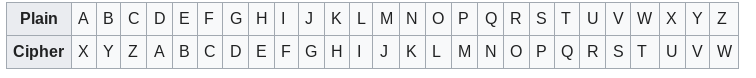
\includegraphics[width = \textwidth]{Screenshot 2024-11-24 22.13.38.png}
\medskip

To do this mathematically, it is easiest to give each letter in the alphabet a number from 1 to 26. Then when this letter comes up in the plaintext, the key can be added or subtracted (depending on whether it is a left or right shift) mod 26 (to loop back to the start of the alphabet if the number is greater than 26 so the letter goes past Z) to produce the new number and corresponding letter for the ciphertext. To implement this computationally, the alphabet can be put in a list where each letter will have an index from 0 to 25.
This can be seen implemented in the function here:
\medskip
% \includegraphics[width = \textwidth]{Screenshot 2024-11-24 22.51.17.png}
\begin{lstlisting}
def caesar_shift(plaintext: str, keyset: str, key: int) -> str:
    ciphertext = ""
    number_of_keys = len(keyset)

    for char in plaintext:
        if char.lower() in keyset:
            char = char.lower()
            index = keyset.index(char)
            new_index = (index + key) % number_of_keys
            char = keyset[new_index]
            ciphertext += char
        else:
            ciphertext += char
    return ciphertext
\end{lstlisting}
\medskip

The Caesar Cipher was a useful way to protect the transfer of information thousands of years ago, when it was relatively new. However, because of its simplicity, people quickly realized that it was very easy to decrypt. This could be done by a brute force method of simply trying all possible keys (adding or subtracting all the numbers from 1 to 25) and seeing which one produced a readable message because the keyset, the set of possible keys, is so small. As shown computationally here, but using a different approach to give each letter numbers as it uses their ASCII value instead of putting them in a list):
\medskip
% \includegraphics[width = \textwidth]{Screenshot 2024-11-24 23.12.36.png}
\begin{lstlisting}
def breakceaser(cypher, keys):
    newplain = ""
    for i in range (0, len(cypher)):
        if ord(cypher[i]) == 32:
            newplain = newplain + chr(32)
        elif ord(cypher[i]) < 97 or ord(cypher[i]) > 122:
            pass
        else:
            num = ord(cypher[i])
            newnum = ((num + keys - 97) % 26) + 97
            newplain = newplain + chr(newnum)
        return newplain      
\end{lstlisting}
Or could be done by trying to figure out the key using frequency analysis, where common letters and words are compared to the cipher text to see what shift would be required to produce them and then this key is tested. This can be seen implemented computationally here: %something to add here%
\\
Therefore, the Caesar Cipher no longer has any use in communication security. However, the encryption step using a key was developed into more complex ciphers such as the Vigenere Cipher.

\subsection{Vigenere Cipher}
The Vigenere Cipher is a more complicated substitution cipher where each letter of the plaintext is encoded with a different Caesar Cipher, determined by the corresponding letter of another word, the key. The plaintext is split into sections each the length of the key. The first letter of the section will be encoded by a Caesar Cipher shift of the numerical value in the alphabet of the first letter in the key. This continues in each section. For example, if the first letter of the plaintext in A and the first letter of the key is E then A will undergo a left-shift of 5 (as E is the 5th letter in the alphabet).\medskip

% To do this practically the corresponding letter of the plaintext and key can be encrypted using the Vigenere square:\medskip

% \includegraphics[width = \textwidth]{Screenshot 2024-11-24 23.37.19.png}
\medskip
To do this computationally the plaintext should be split into sections (each the same length as the key length). This can be done by keeping a counter that increments each time a letter is Caesar shifted and if it gets larger than the length of the keyword will go back to 0. This counter can be used as the index to use the correct letter of the keyword to use for the Caesar shift. This can be seen being implemented here:\medskip

% \includegraphics[width = \textwidth]{Screenshot 2024-11-24 23.44.31.png}
\begin{lstlisting}
def vigenere_cipher(plaintext: str, keyword: str) -> str:
    ciphertext = ""
    current_cipher_index = 0
    length_of_keyword = len(keyword)

    for char in plaintext:
        if char.lower() in alphabet:
            if current_cipher_index > length_of_keyword - 1:
                current_cipher_index = 0
            local_key = alphabet.index(keyword[current_cipher_index].lower())
            ciphertext += caesar_shift(char, alphabet, local_key)
            current_cipher_index += 1
        else:
            ciphertext += char

    return ciphertext
\end{lstlisting}
\medskip
This method of encryption is much more secure than the Caesar Cipher as each letter could be shifted by any of the 26 letters so without the key it is very hard to work out how to decrypt each letter. However, due to the repetitive nature of the key it can sometimes be possible to break this cipher.\medskip

One way this can be done by looking for repeated sections in the ciphertext and seeing how far apart they are from each other. The key length can then be assumed to be a factor of this distance. For example in the following ciphertext:\medskip

% \includegraphics[width = \textwidth]{Screenshot 2024-11-25 10.51.15.png}
\[\bm{CSASTP}KVSIQUTGQU\bm{CSASTP}IUAQJB\]
\medskip
The substring "CSASTP" is 16 letters apart. Therefore, it can be assumed that these repeated segments represent the same plaintext segments and so the key length is a factor of 16 (16,8,4,2,1). This is easier to implement with longer plaintexts as there are likely to be more repeated segments. The key length can then be guessed by looking at common factors of the distances between all the repeated segments. This method to guess the key length is known as 'Kasiski analysis' \cite{kasiski} which we can see implemented here:\medskip

% \includegraphics[width = \textwidth]{Screenshot 2024-11-26 22.33.17.png}
\begin{lstlisting}
def kasiski_analyser(ciphertext: str) -> list[int]:
    string_to_analyse = ""
    for char in ciphertext:
        if char != " ":
            string_to_analyse += char # remove spaces

    repeated_substrings = {} #substring: [positions]

    for substring_length in range(3, 12):
        for i in range(len(string_to_analyse) - substring_length - 1):
            potential_repeat = string_to_analyse[i:i+substring_length]

            positions = []
            index = 0
            while index < len(string_to_analyse):
                index = string_to_analyse.find(potential_repeat, index)
                if index == -1:
                    break
                positions.append(index)
                index += substring_length

            if len(positions) > 1 and potential_repeat not in repeated_substrings:
                if positions[0] % substring_length == positions[1] % substring_length:
                    repeated_substrings[potential_repeat] = positions

    distances = []
    for sub in repeated_substrings:
        distances.append(repeated_substrings[sub][1] - repeated_substrings[sub][0])

    d_factors = []
    for distance in distances:
        d_factors += factors(distance)
        # factors(n) returns a set of the factors of n
 
    # remove 1
    d_factors = [num for num in d_factors if num != 1]
    # sort into frequency
    d_factors = [i for items, c in Counter(d_factors).most_common() for i in [items] * c]
    # remove duplicates
    d_factors = list(dict.fromkeys(d_factors))
    # adds back one if the list is empty
    d_factors = [1] if d_factors == [] else d_factors

    return distances_factors
\end{lstlisting}
\medskip

Once the length of the key is guessed, the ciphertext can be split into many columns, with each column corresponding to one letter of the key. Frequency analysis can then  be used on each column where the most common letters in that column are compared to the most common letters in the english language to try and find the value of the Caesar shift in that column. This method (using both frequency analysis and Kasiski analysis) can be seen implemented here:\medskip

Overall, the Caesar Cipher is a very primitive cipher that is very easy to crack. The Vigenere cipher is more advanced but for longer plaintexts can almost always be solved by using frequency analysis. Therefore, neither of these methods are used in modern day communication.

\section{Programme of Work}
\subsection{Meeting 1 (16.10.24)}
In our first meeting we were introduced to classical cryptography with the Caesar and Vigenere ciphers. We were also given a small introduction to RSA encryption. We were tasked with programming and solving the Caesar and Vigenere ciphers and investigating RSA encryption in python. The Vigenere cipher was much more difficult to decode than the Caesar cipher, as the size of the Caesar cipher's keyset is 26 while the size of the keyset of the the Vigenere cipher is $ 26^n $ where n is the length of the ciphertext. We first tried to decode it using the Index of Coincidence \cite{ioc} of columns of the ciphertext, which can be used to guess the length of the keyword, after which frequency analysis can be applied. This method was unsuccessful, and we then opted to Kasiski analysis \cite{kasiski}, which was much more succesful. Following this, we were able to decode the Vigenere cipher to a large degree of accuracy - on certain ciphertexts, particular of a small length, have a lower chance of being correctly decoded due to the nature of the Vigenere cipher, being easier to decode with larger texts.

\subsection{Meeting 2 (6.11.24)}
During our second meeting, Mr Savage reviewed our code and guided us on making it more pythonic and instructed us to add docstrings. We also discussed the specific details of our long-term goal of our project, and we decided to target quantum computers, as we believe that these pose the greatest threat to quantum cryptography. After the meeting, we updated our code according to Mr Savage's guidelines, and proceeded to research quantum algorithms. RSA encryption's security depends on the hardness of integer factorisation, (which on classical computers has time complexity big O, while quantum computers have time complexity big O), due to Shor's algorithm, which can theoretically be used to factorise integers very quickly once there are powerful enough quantum computers (insert value of how powerful). We also began to research 'learning with errors', which is the basis of many quantum-resistant algorithms \cite{LWE}.

\subsection{Meeting 3 (20.11.24)}
During our third meeting, Mr Savage provided us with a Github repository of a lattice-based learning with errors cipher, with guidance on what research we could pursue.


\bibliographystyle{unsrt}
\bibliography{references.bib}

\end{document}
